\documentclass{beamer}
\usepackage[utf8]{inputenc}
\usepackage[UKenglish]{babel}
\usepackage[UKenglish]{isodate}
\usepackage[style=verbose]{biblatex}
\usepackage{amsmath}
\usepackage{mathtools}
\usepackage{tikz}

\usetheme{CambridgeUS}

\usetikzlibrary{shapes}
\usetikzlibrary{arrows}
\usetikzlibrary{arrows.meta}

\beamertemplatenavigationsymbolsempty
\addbibresource{talk.bib}
\DeclareRobustCommand{\stirling}{\genfrac\{\}{0pt}{}}

\author{Paulius Dilkas}
\title[Empowering Domain Recursion]{Empowering Domain Recursion in Symmetric Weighted First-Order Model Counting}
\date{}

\begin{document}
\addtobeamertemplate{block begin}{\setlength\abovedisplayskip{0pt}}

\maketitle

\begin{frame}{Overview}
  \begin{block}{Hypothesis}
    Partial injections can be counted in polynomial time using (a modification of) \textsc{ForcLift}.
  \end{block}
  \begin{block}{Key Ideas \& Progress}
    \begin{itemize}
    \item[\textcolor{green}{100\%}] Support for cycles in circuits
    \item[\textcolor{green}{95\%}] Transforming $X \ne x$ constraints into domain reductions $\Delta' \coloneqq \Delta \setminus \{ x \}$
    \item[\textcolor{green}{95\%}] A less restrictive version of domain recursion
    \item[\textcolor{orange}{90\%}] A hybrid search algorithm
    \item[\textcolor{red}{0\%}] Complexity identification
    \end{itemize}
  \end{block}
\end{frame}

\begin{frame}{Search}
  \begin{definition}
    A \alert{partial solution} (i.e., a search node) is a tuple consisting of:
    \begin{itemize}
    \item a partial circuit, i.e., a \textsc{ForcLift}-style DAG,
      \begin{itemize}
      \item Each node type has a predefined out-degree.
      \item Some of them may be `arcs to nothing'.
      \end{itemize}
    \item a cache (i.e., a formula $\to$ node hashmap), used to identify opportunities for recursion,
    \item a list of formulas that still need to be compiled, listed in a particular order.
    \end{itemize}
  \end{definition}
  % Sink and non-sink rules
\end{frame}

\begin{frame}{Search}
  Some rules are applied in a greedy manner:
  \begin{itemize}
  \item identifying the current formula as something that's already been compiled using the cache;
  \item sink nodes: tautologies, contradictions, unit clauses;
  \item some formula-simplifying rules;
  \item unit propagation.
  \end{itemize}
  And some rules are used to branch out into several possibilities:
  \begin{itemize}
  \item independent subtheories,
  \item shattering,
  \item ground decomposition,
  \item inclusion-exclusion,
  \item independent partial grounding,
  \item counting,
  \item (my version of) domain recursion.
  \end{itemize}
\end{frame}

\begin{frame}{WFOMC: State of the Art}
  I'm excluding techniques that are restricted to two variables and purely
  theoretical results.
  \begin{enumerate}
  \item \cite{DBLP:conf/nips/KazemiKBP16}
    \begin{itemize}
    \item generic domain recursion (implementation unavailable)
    \end{itemize}
  \item \alert{Forclift}: \cite{DBLP:conf/ijcai/BroeckTMDR11}
    \begin{itemize}
    \item somewhat restrictive but well-developed
    \end{itemize}
  \item \alert{L2C}: \cite{DBLP:conf/kr/KazemiP16}
    \begin{itemize}
    \item very basic
    \end{itemize}
  \item \alert{Alchemy}: \cite{DBLP:conf/aaai/DomingosKPRS06}
    \begin{itemize}
    \item old, mostly focused on approximations
    \end{itemize}
  \end{enumerate}
\end{frame}

\begin{frame}{Counting Injections}
  %% \cite{stanley2011enumerative}
  %% \begin{block}{Functions $M \to N$ (let $|M| = m$ and $|N| = n$)}
  %%   Theory:
  %%   \begin{align*}
  %%     \forall x \in M. \forall y, z \in N. &P(x, y) \land P(x, z) \Rightarrow y=z \\
  %%     \forall x \in M. \exists y \in N. &P(x, y)
  %%   \end{align*}
  %%   Answer: $n^m$.
  %% \end{block}
  Theory:
  \begin{align*}
    \forall x \in M. \forall y, z \in N. &P(x, y) \land P(x, z) \Rightarrow y=z \\
    \forall x \in M. \exists y \in N. &P(x, y) \\
    \forall w, x \in M. \forall y \in N. &P(w, y) \land P(x, y) \Rightarrow w=x
  \end{align*}
  Answer: $n^{\underline{m}} = n \cdot (n-1)\cdots(n-m+1)$ if $m \le n$ and $0$ otherwise (for positive $m$ and $n$).
\end{frame}

\begin{frame}
  \begin{block}{One answer}
    \[
    f(m, n) = \sum_{k=0}^m \binom{m}{k}(-1)^{m-k}g(k, n),
    \]
    where
    \[
    g(k, n) =
    \begin{cases}
      1 & \text{if } k = 0 \\
      \sum_{l=0}^n [l < 2]g(k-1, n-l) & \text{otherwise.}
    \end{cases}
    \]
  \end{block}
  \begin{block}{Another answer (almost found by Forclift)}
    (The missing parts are highlighted) Same $f$ and...
    \[
    g(m, n) =
    \begin{cases}
      1 & \text{if } m = 0 \\
      \alert{n+1} & \alert{\text{if } m = 1} \\
      \sum_{k=0}^{\min\{n, 1\}} \sum_{l=0}^{\min\{n-k, 1\}} \alert{\frac{n!}{(n-m-l)!}} g(m-2, n-m-l) & \text{otherwise.}
    \end{cases}
    \]
  \end{block}
\end{frame}

\begin{frame}{Counting (Unweighted) Functions: Currently Unliftable (2)}
  \begin{block}{Surjections}
    Theory:
    \begin{align*}
      \forall x \in M. \forall y, z \in N. &P(x, y) \land P(x, z) \Rightarrow y=z \\
      \forall x \in M. \exists y \in N. &P(x, y) \\
      \alert{\forall y \in N. \exists x \in M.} &\alert{P(x, y)}
    \end{align*}
    Answer: $n!\stirling{m}{n} = \sum_{i=0}^n (-1)^i\binom{n}{i}(n-i)^m$.
  \end{block}
\end{frame}

\begin{frame}{Counting (Unweighted) Functions: Currently Unliftable (3)}
  \begin{block}{Partial functions}
    Theory: $\forall x \in M. \forall y, z \in N. P(x, y) \land P(x, z)
    \Rightarrow y=z$

    Answer: $(n+1)^m$.
  \end{block}
  \begin{block}{Partial injections}
    Theory:
    \begin{align*}
      \forall x \in M. \forall y, z \in N. &P(x, y) \land P(x, z) \Rightarrow y=z \\
      \forall w, x \in M. \forall y \in N. &P(w, y) \land P(x, y) \Rightarrow w=x
    \end{align*}
    My answer: $\sum_{k=0}^{\min\{m, n\}} k!\binom{m}{k}\binom{n}{k}$.

    \pause
    \alert{Answer found by Forclift:}
    \[
    f(m, n) =
    \begin{cases}
      1 & \text{if } m = 0 \\
      \sum_{k=0}^n \binom{n}{k} [k < 2] f(m-1, k) & \text{otherwise.}
    \end{cases}
    \]
    (exponential...)
  \end{block}
\end{frame}

\begin{frame}{Conceptual Plan of Action}
  \centering
  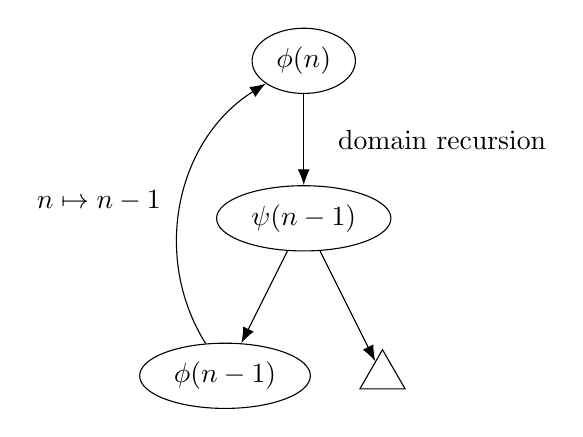
\begin{tikzpicture}[triangle/.style = {regular polygon, regular polygon sides=3}]
    \node[draw,ellipse] (a) at (0, 0) {$\phi(n)$};
    \node[draw,ellipse] (b) at (0, -2) {$\psi(n-1)$};
    \node[draw,ellipse] (c) at (-1, -4) {$\phi(n-1)$};
    \node[draw,triangle] (d) at (1, -4) {};
    \draw[-{Latex[length=2mm]}] (a) -- (b) node [midway,xshift=50] {domain recursion};
    \draw[-{Latex[length=2mm]}] (b) -- (c);
    \draw[-{Latex[length=2mm]}] (b) -- (d);
    \draw[-{Latex[length=2mm]}] (c) to [bend left=45] node [midway,xshift=-30] () {$n \mapsto n-1$} (a);
  \end{tikzpicture}
\end{frame}

\begin{frame}{Remarks on the Implementation}
  \begin{itemize}
  \item WMC computation now loops over the graph.
  \item We propagate information (e.g., for smoothing) in reverse until convergence.
  \item Need a good way to recognise equivalent/isomorphic theories.
  \item Need to be careful about the order of operations:
    \begin{itemize}
    \item Create a (half-empty) vertex $v$.
    \item Add it to the cache.
    \item Recurse on its direct successors $S$.
    \item Add the edges from $v$ to $S$.
    \item After the graph is constructed, propagate information through the
      graph that would otherwise cause infinite loops.
    \end{itemize}
  \end{itemize}
\end{frame}

\begin{frame}{Domain Size Comparisons}
  \begin{block}{$|N| < 2$ (Forclift can already do this!)}
    \[
    \phi \equiv \forall x, y \in N \text{ s.t. } x \ne y\text{, } P,
    \]
    where $w(P) = 0$. The algebraic (multiplicative) contribution of $\phi$ is $w(P)^{\mathrm{gr}(\phi)}$.
    \begin{itemize}
    \item If $|N| \ge 2$, then $\mathrm{gr}(\phi) > 0$, and so $0^{\mathrm{gr}(\phi)} = 0$.
    \item If $|N| < 2$, then we get $0^0 = 1$.
    \item Of course, 2 can be replaced by any other positive integer.
    \end{itemize}
  \end{block}
  \pause
  \begin{block}{$m < n$ (possible, but a bit complicated)}
    \[
    f(m, n) = \begin{cases}
      0 & \text{if } n = 0 \\
      1 & \text{if } m = 0 \text{ and } n > 0 \\
      f(m-1, n-1) & \text{otherwise.}
    \end{cases}
    \]
  \end{block}
\end{frame}

\begin{frame}{Bijections}
  \begin{align*}
    \forall x \in M. \forall y, z \in N. &P(x, y) \land P(x, z) \Rightarrow y=z \\
    \forall x \in M. \exists y \in N. &P(x, y) \\
    \forall w, x \in M. \forall y \in N. & P(w, y) \land P(x, y) \Rightarrow w=x \\
    \forall y \in N. \exists x \in M. & P(x, y)
  \end{align*}
  Answer: $n!$ if $m=n$ and zero otherwise.
\end{frame}

\begin{frame}{Bijections: a linear answer found by Forclift}
  \begin{align*}
    f(m, n) &= - f(m, n-1) + \sum_{k=0}^m \binom{m}{k}[k < 2]f(m - k, n - 1) \\
    &= - f(m, n-1) + f(m, n - 1) + m \times f(m - 1, n - 1) \\
    &= m \times f(m - 1, n - 1)
  \end{align*}
  This works if supplied with the right base cases:
  \begin{align*}
    f(0, 0) &= 1, \\
    f(m, 0) &= 0 \text{ (for all $m > 0$),} \\
    f(0, n) &= 0 \text{ (for all $n > 0$).}
  \end{align*}
\end{frame}

\end{document}
